\section{\label{sec:gcol:examples}Examples}

To demonstrate the operation of the \gls{cps} algorithm in a 3-colouring context, this \namecref{sec:gcol:examples} provides a working example using the graph in \cref{fig:gcol:examplegraph}, and a failing example where no successful 3-colouring is possible using the graph in \cref{fig:gcol:examplegraphnosol}.

\begin{figure}
    \centering
    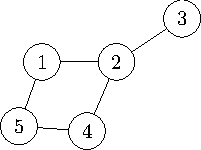
\includegraphics[width=0.4\textwidth]{chapters/gcol/figs/examplegraph1-figure2.pdf}
    \caption[Example graph with at least one possible three-colouring solution]{Example undirected graph with at least one possible three-colouring solution (in fact, this graph is also potentially 2-colourable, and the \glspl{cps} might select such a solution).}
    \label{fig:gcol:examplegraph}
\end{figure}

\begin{figure}
    \centering
    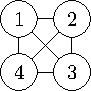
\includegraphics[width=0.2\textwidth]{chapters/gcol/figs/examplegraph1-figure3.pdf}
    \caption{Example graph with no valid three-colouring solutions.}
    \label{fig:gcol:examplegraphnosol}
\end{figure}

\subsection{Successful Example}

For the graph in \cref{fig:gcol:examplegraph}, begin with a single \gls{tlc} situated in the environment and in state \(s_1\).  From the hypothetical set of nodes \(V = \{1, 2, 3, 4, 5\}\),  derive the \gls{functor}
\[V' = \cpfunc{v}{\cpfunc{n}{1}~\cpfunc{n}{2}~\cpfunc{n}{3}~\cpfunc{n}{4}~\cpfunc{n}{5}}.\]
Define also the object set
\[E' = \cpset{\cpfunc{e}{\cpfunc{n}{1} \, \cpfunc{n}{2}},~\cpfunc{e}{\cpfunc{n}{1} \, \cpfunc{n}{5}},~\cpfunc{e}{\cpfunc{n}{2} \, \cpfunc{n}{3}},~\cpfunc{e}{\cpfunc{n}{2} \, \cpfunc{n}{4}},~\cpfunc{e}{\cpfunc{n}{4} \, \cpfunc{n}{5}}}\]
representing the edges of the graph, as well as the set of colour objects
\(K' = \cpset{\cpfunc{k}{r},~\cpfunc{k}{g},~\cpfunc{k}{b}}\),
representing in this case the colours red, green and blue.  These sets of objects are all immediately inside the \gls{tlc}, along with \(\cpfunc{s}{1}\) to select node 1 at the beginning of the process, as shown in \cref{objs:gcol:obj1}.

This beginning state, except for the choice of node label inside the \(s\) object, is mandatory, but all following discussion in this subsection is just one possible execution, due to the non-deterministic selection of colours during application of \cpruleref{rule:gcol:rules:init} and \cpruleref{rule:gcol:rules:endsucc}.

\begin{cpobjectsfloat}
\begin{cpobjects}
\cpobjectsline{\cpfunc{e}{\cpfunc{n}{1} \, \cpfunc{n}{2}} \; \cpfunc{e}{\cpfunc{n}{1} \, \cpfunc{n}{5}} \; \cpfunc{e}{\cpfunc{n}{2} \, \cpfunc{n}{3}} \; \cpfunc{e}{\cpfunc{n}{2} \, \cpfunc{n}{4}} \; \cpfunc{e}{\cpfunc{n}{4} \, \cpfunc{n}{5}}}
\cpobjectsline{ \cpfunc{k}{r} \, \cpfunc{k}{g} \, \cpfunc{k}{b} \quad \cpfunc{s}{1} \quad \cpfunc{v}{\cpfunc{n}{1} \; \cpfunc{n}{2} \; \cpfunc{n}{3} \; \cpfunc{n}{4} \; \cpfunc{n}{5}}}
\end{cpobjects}
\caption{\label{objs:gcol:obj1}Initial set of objects in the \gls{tlc}, for \cref{fig:gcol:examplegraph}.}
\end{cpobjectsfloat}

From this starting state, \cpruleref{rule:gcol:rules:init} is applied, choosing node 1 to start the process with, and selecting red as its colouring.  This creates the standard \(b\) object.  No other rules are applicable at this point, as the \gls{tlc} started in state \(s_1\).  The application of this rule leaves the \gls{tlc} in state \(s_2\).  \cpRuleref{rule:gcol:rules:init} will henceforth be inapplicable, as the rules provide no way to revert to state \(s_1\).

At the next step, \cpruleref{rule:gcol:rules:endsucc} is checked but found inapplicable, as at this point the \(v\) object inside the only \(b\) object will \emph{not} be empty, instead containing \(\cpfunc{v}{\cpfunc{n}{2} \, \cpfunc{n}{3} \, \cpfunc{n}{4} \, \cpfunc{n}{5}}\).  \cpRuleref{rule:gcol:rules:loop}, conversely, is applicable and thus can generate further new \(b\) objects.  In this instance, two edges exist from node 1 to other nodes (2 and 5 specifically), meaning that both choices can apply, generating new \(b\) objects containing the legal  colourings.  Both nodes are chosen to connect to, but there are only two other possible colourings to choose here, as red is currently blocked due to it being selected for the first \(b\) object.  This leads to the creation of four (two colours times two nodes) new \(b\) objects \(\cpfunc{b}{\cpfunc{m}{\cpfunc{n}{1} \, \cpfunc{c}{r}}\allowbreak ~\cpfunc{m}{\cpfunc{n}{2} \, \cpfunc{c}{g}}\allowbreak ~\cpfunc{v}{\cpfunc{n}{3}~ \cpfunc{n}{4}~ \cpfunc{n}{5}}}\), \(\cpfunc{b}{\cpfunc{m}{\cpfunc{n}{1} \, \cpfunc{c}{r}}\allowbreak ~\cpfunc{m}{\cpfunc{n}{5} \, \cpfunc{c}{b}}\allowbreak ~\cpfunc{v}{\cpfunc{n}{2}~ \cpfunc{n}{3}~ \cpfunc{n}{4}}}\) etc.

Simultaneously, \cpruleref{rule:gcol:rules:loopclean} is applied to sweep away the pre-existing initial \(b\) object.  \cpRuleref{rule:gcol:rules:endfail} is not applicable because a state transition to state \(s_2\) has already been selected by application of Rules \cpruleref*{rule:gcol:rules:loop} and \cpruleref*{rule:gcol:rules:loopclean}, and thus a transition to state \(s_4\) is invalid.  \Cref{objs:gcol:obj2} lists the objects in the \gls{tlc} at the end of this step.

\begin{cpobjectsfloat}
\begin{cpobjects}
    \cpobjectsline{\cpfunc{e}{\cpfunc{n}{1} \, \cpfunc{n}{2}} \dots \cpfunc{e}{\cpfunc{n}{4} \, \cpfunc{n}{5}} \quad \cpfunc{k}{r} \, \cpfunc{k}{g} \, \cpfunc{k}{b}
}
\cpobjectsline{
    \cpfunc{b}{\cpfunc{m}{\cpfunc{n}{1} \, \cpfunc{c}{r}}~\cpfunc{m}{\cpfunc{n}{2} \, \cpfunc{c}{g}}~\cpfunc{v}{\cpfunc{n}{3}~ \cpfunc{n}{4}~ \cpfunc{n}{5}}}
}
\cpobjectsline{
    \cpfunc{b}{\cpfunc{m}{\cpfunc{n}{1} \, \cpfunc{c}{r}}~\cpfunc{m}{\cpfunc{n}{2} \, \cpfunc{c}{b}}~\cpfunc{v}{\cpfunc{n}{3}~ \cpfunc{n}{4}~ \cpfunc{n}{5}}}
}
\cpobjectsline{
    \cpfunc{b}{\cpfunc{m}{\cpfunc{n}{1} \, \cpfunc{c}{r}}~\cpfunc{m}{\cpfunc{n}{5} \, \cpfunc{c}{g}}~\cpfunc{v}{\cpfunc{n}{2}~ \cpfunc{n}{3}~ \cpfunc{n}{4}}}
}
\cpobjectsline{
    \cpfunc{b}{\cpfunc{m}{\cpfunc{n}{1} \, \cpfunc{c}{r}}~\cpfunc{m}{\cpfunc{n}{5} \, \cpfunc{c}{b}}~\cpfunc{v}{\cpfunc{n}{2}~ \cpfunc{n}{3}~ \cpfunc{n}{4}}}
}
\end{cpobjects}
\caption[Objects in the \gls{tlc} after the second step, for \cref{fig:gcol:examplegraph}]{\label{objs:gcol:obj2}Objects in the \gls{tlc} after the second step (\ie{} after one application of Rules \cpruleref*{rule:gcol:rules:loop} and \cpruleref*{rule:gcol:rules:loopclean}) for \cref{fig:gcol:examplegraph}.}
\end{cpobjectsfloat}

The next step proceeds almost identically to the previous one, except that there are more new objects created (see \cref{objs:gcol:obj3}).  At the previous step, the edges both between node 1 and node 5, and node 1 and node 2, were explored.  In this next step, edges between node 1 and node 5, node 1 and node 2 (where these edges were not explored previously for a given \(b\) object), node 5 and node 4, and node 2 and node 3 are all explored, with all objects that will not have direct colour conflicts instantiated as per \cpruleref{rule:gcol:rules:loop}.

\begin{cpobjectsfloat}
\begin{cpobjects}
    \cpobjectsline{\cpfunc{e}{\cpfunc{n}{1} \, \cpfunc{n}{2}} \dots \cpfunc{e}{\cpfunc{n}{4} \, \cpfunc{n}{5}} \quad \cpfunc{k}{r} \, \cpfunc{k}{g} \, \cpfunc{k}{b}}
%    
    \cpobjectsline{
        \cpfunc{b}{\cpfunc{m}{\cpfunc{n}{1} \, \cpfunc{c}{r}}~\cpfunc{m}{\cpfunc{n}{2} \, \cpfunc{c}{g}}~\cpfunc{m}{\cpfunc{n}{5} \, \cpfunc{c}{g}}~\cpfunc{v}{\cpfunc{n}{3}~ \cpfunc{n}{4}}}
    }
    \cpobjectsline{
        \cpfunc{b}{\cpfunc{m}{\cpfunc{n}{1} \, \cpfunc{c}{r}}~\cpfunc{m}{\cpfunc{n}{2} \, \cpfunc{c}{g}}~\cpfunc{m}{\cpfunc{n}{5} \, \cpfunc{c}{b}}~\cpfunc{v}{\cpfunc{n}{3}~ \cpfunc{n}{4}}}
    }
    \cpobjectsline{
        \vdots
    }
    \cpobjectsline{
        \cpfunc{b}{\cpfunc{m}{\cpfunc{n}{1} \, \cpfunc{c}{r}}~\cpfunc{m}{\cpfunc{n}{2} \, \cpfunc{c}{b}}~\cpfunc{m}{\cpfunc{n}{3} \, \cpfunc{c}{r}}~\cpfunc{v}{\cpfunc{n}{4}~ \cpfunc{n}{5}}}
    }
    \cpobjectsline{
        \cpfunc{b}{\cpfunc{m}{\cpfunc{n}{1} \, \cpfunc{c}{r}}~\cpfunc{m}{\cpfunc{n}{2} \, \cpfunc{c}{b}}~\cpfunc{m}{\cpfunc{n}{3} \, \cpfunc{c}{g}}~\cpfunc{v}{\cpfunc{n}{4}~ \cpfunc{n}{5}}}
    }
\end{cpobjects}
\caption[Objects in the \gls{tlc} after the third step, for \cref{fig:gcol:examplegraph}]{\label{objs:gcol:obj3}Objects in the \gls{tlc} after the third step for \cref{fig:gcol:examplegraph}.  There will be some identical objects here which have been created independently.}
\end{cpobjectsfloat}

At the fourth step, many further objects are created, some of which are listed in \cref{objs:gcol:obj4}.  The key difference between this step and the previous one is that the final \gls{inhibitor} on \cpruleref{rule:gcol:rules:loop} plays a much greater role.  At this step, many of the potential instantiations of new node and colouration selections will include conflicts between the newly selected node and colour, and one or more of the node and colour selections made earlier.  The final \gls{inhibitor} prevents instantiation of these choices, avoiding threats to correctness.  An alternative solution to the problem would be to include another following step, where those invalid instantiations are detected and removed, but the \gls{inhibitor} makes this unnecessary.  

\begin{cpobjectsfloat}
\begin{cpobjects}
    
    \cpobjectsline{\cpfunc{e}{\cpfunc{n}{1} \, \cpfunc{n}{2}} \dots \cpfunc{e}{\cpfunc{n}{4} \, \cpfunc{n}{5}} \quad \cpfunc{k}{r} \, \cpfunc{k}{g} \, \cpfunc{k}{b}}
    
    \cpobjectsline{\cpfunc{b}{\cpfunc{m}{\cpfunc{n}{1} \, \cpfunc{c}{r}}~\cpfunc{m}{\cpfunc{n}{5} \, \cpfunc{c}{g}}~\cpfunc{m}{\cpfunc{n}{4} \, \cpfunc{c}{r}}~\cpfunc{m}{\cpfunc{n}{2} \, \cpfunc{c}{g}}~\cpfunc{v}{\cpfunc{n}{3}}}}
    
    \cpobjectsline{\cpfunc{b}{\cpfunc{m}{\cpfunc{n}{1} \, \cpfunc{c}{r}}~\cpfunc{m}{\cpfunc{n}{5} \, \cpfunc{c}{g}}~\cpfunc{m}{\cpfunc{n}{4} \, \cpfunc{c}{r}}~\cpfunc{m}{\cpfunc{n}{2} \, \cpfunc{c}{b}}~\cpfunc{v}{\cpfunc{n}{3}}}}
    
    \cpobjectsline{\vdots}
    
    \cpobjectsline{\cpfunc{b}{\cpfunc{m}{\cpfunc{n}{1} \, \cpfunc{c}{r}}~\cpfunc{m}{\cpfunc{n}{2} \, \cpfunc{c}{b}}~\cpfunc{m}{\cpfunc{n}{3} \, \cpfunc{c}{g}}~\cpfunc{m}{\cpfunc{n}{5} \, \cpfunc{c}{g}}~\cpfunc{v}{\cpfunc{n}{4}}}}
    
    \cpobjectsline{\cpfunc{b}{\cpfunc{m}{\cpfunc{n}{1} \, \cpfunc{c}{r}}~\cpfunc{m}{\cpfunc{n}{2} \, \cpfunc{c}{b}}~\cpfunc{m}{\cpfunc{n}{3} \, \cpfunc{c}{g}}~\cpfunc{m}{\cpfunc{n}{5} \, \cpfunc{c}{b}}~\cpfunc{v}{\cpfunc{n}{4}}}}
    
\end{cpobjects}
\caption[Objects in the \gls{tlc} after the fourth step, for \cref{fig:gcol:examplegraph}]{\label{objs:gcol:obj4}Objects in the \gls{tlc} after the fourth step for \cref{fig:gcol:examplegraph}.}
\end{cpobjectsfloat}

Step 5 proceeds analogously.  At the end of step 5 a number of \(b\) objects which contain valid colourings of the whole graph will be present inside the \gls{tlc}.  At the sixth step, \cpruleref{rule:gcol:rules:endsucc} will detect this by the fact that said objects will contain empty \(v\) \glspl{functor}.  For example, \cref{objs:gcol:obj6} shows some of the potential solutions that could be generated, reflecting the state of the system at the end of the fifth step.  In fact, the first potential solution shows that in this case it is possible to completely and validly colour this graph using only two colours.  This solution may or may not be chosen when \cpruleref{rule:gcol:rules:endsucc} is applied.  At the sixth step, \cpruleref{rule:gcol:rules:endsucc} will select one of the possible solutions and emit it to the environment.  The \gls{tlc} will also transition to state \(s_3\), signalling that the process succeeded.

\begin{cpobjectsfloat}
\begin{cpobjects}

    \cpobjectsline{\cpfunc{e}{\cpfunc{n}{1} \, \cpfunc{n}{2}} \dots \cpfunc{e}{\cpfunc{n}{4} \, \cpfunc{n}{5}} \quad \cpfunc{k}{r} \, \cpfunc{k}{g} \, \cpfunc{k}{b}}
    
    \cpobjectsline{\cpfunc{b}{\cpfunc{m}{\cpfunc{n}{1} \, \cpfunc{c}{r}}~\cpfunc{m}{\cpfunc{n}{5} \, \cpfunc{c}{g}}~\cpfunc{m}{\cpfunc{n}{4} \, \cpfunc{c}{r}}~\cpfunc{m}{\cpfunc{n}{2} \, \cpfunc{c}{g}}~\cpfunc{m}{\cpfunc{n}{3} \, \cpfunc{c}{r}}~\cpfunc{v}{\cpempty}}}
    
    \cpobjectsline{\cpfunc{b}{\cpfunc{m}{\cpfunc{n}{1} \, \cpfunc{c}{r}}~\cpfunc{m}{\cpfunc{n}{5} \, \cpfunc{c}{g}}~\cpfunc{m}{\cpfunc{n}{4} \, \cpfunc{c}{r}}~\cpfunc{m}{\cpfunc{n}{2} \, \cpfunc{c}{g}}~\cpfunc{m}{\cpfunc{n}{3} \, \cpfunc{c}{b}}~\cpfunc{v}{\cpempty}}}
    
            \cpobjectsline{\vdots}
            
    \cpobjectsline{\cpfunc{b}{\cpfunc{m}{\cpfunc{n}{1} \, \cpfunc{c}{r}}~\cpfunc{m}{\cpfunc{n}{2} \, \cpfunc{c}{b}}~\cpfunc{m}{\cpfunc{n}{3} \, \cpfunc{c}{g}}~\cpfunc{m}{\cpfunc{n}{5} \, \cpfunc{c}{g}}~\cpfunc{m}{\cpfunc{n}{4} \, \cpfunc{c}{r}}~\cpfunc{v}{\cpempty}}}
    
    \cpobjectsline{\cpfunc{b}{\cpfunc{m}{\cpfunc{n}{1} \, \cpfunc{c}{r}}~\cpfunc{m}{\cpfunc{n}{2} \, \cpfunc{c}{b}}~\cpfunc{m}{\cpfunc{n}{3} \, \cpfunc{c}{g}}~\cpfunc{m}{\cpfunc{n}{5} \, \cpfunc{c}{g}}~\cpfunc{m}{\cpfunc{n}{4} \, \cpfunc{c}{r}}~\cpfunc{v}{\cpempty}}}
\end{cpobjects}
\caption{\label{objs:gcol:obj6}Objects in the \gls{tlc} after the fifth step, for \cref{fig:gcol:examplegraph}.}
\end{cpobjectsfloat}

% ------------------------------------------------

\subsection{\label{sec:gcol:examplefail}Failing Example}
This \namecref{sec:gcol:examplefail} steps through the execution of the algorithm when there is no possible valid 3-colouring solution, using the graph depicted in \cref{fig:gcol:examplegraphnosol}.  The system begins with the objects depicted in \cref{objs:gcol:objn1}.

\begin{cpobjectsfloat}
\begin{cpobjects}

    \cpobjectsline{\cpfunc{e}{\cpfunc{n}{1} \, \cpfunc{n}{2}} \; \cpfunc{e}{\cpfunc{n}{1} \, \cpfunc{n}{3}} \; \cpfunc{e}{\cpfunc{n}{1} \, \cpfunc{n}{4}} \; \cpfunc{e}{\cpfunc{n}{2} \, \cpfunc{n}{3}} \; \cpfunc{e}{\cpfunc{n}{2} \, \cpfunc{n}{4}} \; \cpfunc{e}{\cpfunc{n}{3} \, \cpfunc{n}{4}}}
    
    \cpobjectsline{\cpfunc{k}{r} \, \cpfunc{k}{g} \, \cpfunc{k}{b} \quad \cpfunc{s}{1}}
    
    \cpobjectsline{\cpfunc{v}{\cpfunc{n}{1}~\cpfunc{n}{2}~\cpfunc{n}{3}~\cpfunc{n}{4}}}
\end{cpobjects}
\caption{\label{objs:gcol:objn1}Initial set of objects in the \gls{tlc}, for \cref{fig:gcol:examplegraphnosol}.}
\end{cpobjectsfloat}

After the first step, the application of \cpruleref{rule:gcol:rules:init}, the objects shown in \cref{objs:gcol:objn2} are inside the \gls{tlc}.  This is not substantively different from the successful example above.  Likewise with the objects present in the cell at the end of the second step, shown in \cref{objs:gcol:objn3}.

\begin{cpobjectsfloat}
\begin{cpobjects}

    \cpobjectsline{\cpfunc{e}{\cpfunc{n}{1} \, \cpfunc{n}{2}} \dots \cpfunc{e}{\cpfunc{n}{3} \, \cpfunc{n}{4}} \quad \cpfunc{k}{r} \, \cpfunc{k}{g} \, \cpfunc{k}{b}}
    
    \cpobjectsline{\cpfunc{b}{\cpfunc{m}{\cpfunc{n}{1} \, \cpfunc{c}{r}}~\cpfunc{v}{\cpfunc{n}{2}~\cpfunc{n}{3}~\cpfunc{n}{4}}}}
\end{cpobjects}
\caption{\label{objs:gcol:objn2}Objects in the \gls{tlc} at the end of step 1, for \cref{fig:gcol:examplegraphnosol}.}
\end{cpobjectsfloat}

\begin{cpobjectsfloat}
\begin{cpobjects}
    
    \cpobjectsline{\cpfunc{e}{\cpfunc{n}{1} \, \cpfunc{n}{2}} \dots \cpfunc{e}{\cpfunc{n}{3} \, \cpfunc{n}{4}} \quad \cpfunc{k}{r} \, \cpfunc{k}{g} \, \cpfunc{k}{b}}
    
    \cpobjectsline{\cpfunc{b}{\cpfunc{m}{\cpfunc{n}{1} \, \cpfunc{c}{r}}~\cpfunc{m}{\cpfunc{n}{2} \, \cpfunc{c}{g}}~\cpfunc{v}{\cpfunc{n}{3}~\cpfunc{n}{4}}}}
    
    \cpobjectsline{\cpfunc{b}{\cpfunc{m}{\cpfunc{n}{1} \, \cpfunc{c}{r}}~\cpfunc{m}{\cpfunc{n}{2} \, \cpfunc{c}{b}}~\cpfunc{v}{\cpfunc{n}{3}~\cpfunc{n}{4}}}}
    
    \cpobjectsline{\cpfunc{b}{\cpfunc{m}{\cpfunc{n}{1} \, \cpfunc{c}{r}}~\cpfunc{m}{\cpfunc{n}{3} \, \cpfunc{c}{g}}~\cpfunc{v}{\cpfunc{n}{2}~\cpfunc{n}{4}}}}
    
    \cpobjectsline{\cpfunc{b}{\cpfunc{m}{\cpfunc{n}{1} \, \cpfunc{c}{r}}~\cpfunc{m}{\cpfunc{n}{3} \, \cpfunc{c}{b}}~\cpfunc{v}{\cpfunc{n}{2}~\cpfunc{n}{4}}}}
    
    \cpobjectsline{\cpfunc{b}{\cpfunc{m}{\cpfunc{n}{1} \, \cpfunc{c}{r}}~\cpfunc{m}{\cpfunc{n}{4} \, \cpfunc{c}{g}}~\cpfunc{v}{\cpfunc{n}{2}~\cpfunc{n}{3}}}}
    
    \cpobjectsline{\cpfunc{b}{\cpfunc{m}{\cpfunc{n}{1} \, \cpfunc{c}{r}}~\cpfunc{m}{\cpfunc{n}{4} \, \cpfunc{c}{b}}~\cpfunc{v}{\cpfunc{n}{2}~\cpfunc{n}{3}}}}

\end{cpobjects}
\caption{\label{objs:gcol:objn3}Objects in the \gls{tlc} at the end of step 2, for \cref{fig:gcol:examplegraphnosol}.}
\end{cpobjectsfloat}

\Cref{objs:gcol:objn4} shows the objects in the \gls{tlc} at the end of step three.  This proceeds in much the same fashion as the previous step, but fully half of the potential instantiations from \cpruleref{rule:gcol:rules:loop} are avoided by the rule's final \gls{inhibitor}, due to inescapable colouration conflicts.

\begin{cpobjectsfloat}
\begin{cpobjects}

    \cpobjectsline{\cpfunc{e}{\cpfunc{n}{1} \, \cpfunc{n}{2}} \dots \cpfunc{e}{\cpfunc{n}{3} \, \cpfunc{n}{4}} \quad \cpfunc{k}{r} \, \cpfunc{k}{g} \, \cpfunc{k}{b}}
    
    \cpobjectsline{\cpfunc{b}{\cpfunc{m}{\cpfunc{n}{1} \, \cpfunc{c}{r}}~\cpfunc{m}{\cpfunc{n}{2} \, \cpfunc{c}{g}}~\cpfunc{m}{\cpfunc{n}{3} \, \cpfunc{c}{b}}~\cpfunc{v}{\cpfunc{n}{4}}}}
    
    \cpobjectsline{\cpfunc{b}{\cpfunc{m}{\cpfunc{n}{1} \, \cpfunc{c}{r}}~\cpfunc{m}{\cpfunc{n}{2} \, \cpfunc{c}{g}}~\cpfunc{m}{\cpfunc{n}{3} \, \cpfunc{c}{b}}~\cpfunc{v}{\cpfunc{n}{4}}}}
    
        \cpobjectsline{\vdots}
        
    \cpobjectsline{\cpfunc{b}{\cpfunc{m}{\cpfunc{n}{1} \, \cpfunc{c}{r}}~\cpfunc{m}{\cpfunc{n}{2} \, \cpfunc{c}{g}}~\cpfunc{m}{\cpfunc{n}{4} \, \cpfunc{c}{b}}~\cpfunc{v}{\cpfunc{n}{3}}}}
    
    \cpobjectsline{\cpfunc{b}{\cpfunc{m}{\cpfunc{n}{1} \, \cpfunc{c}{r}}~\cpfunc{m}{\cpfunc{n}{2} \, \cpfunc{c}{g}}~\cpfunc{m}{\cpfunc{n}{4} \, \cpfunc{c}{b}}~\cpfunc{v}{\cpfunc{n}{3}}}}
    
\end{cpobjects}
\caption{\label{objs:gcol:objn4}Objects in the \gls{tlc} at the end of step 3, for \cref{fig:gcol:examplegraphnosol}.}
\end{cpobjectsfloat}

Finally, \cref{objs:gcol:objn5} shows the objects in the \gls{tlc} as at the end of step 4.  Due to the fully connected nature of the graph in \cref{fig:gcol:examplegraphnosol}, every possible solution will contain at least one instance of proposed contiguous colouration, thus making every possible solution invalid.  This means that \cpruleref{rule:gcol:rules:loop} will not create any new \(b\) objects, while \cpruleref{rule:gcol:rules:loopclean} will remove the pre-existing ones.

\begin{cpobjectsfloat}
\begin{cpobjects}

    \cpobjectsline{\cpfunc{e}{\cpfunc{n}{1} \, \cpfunc{n}{2}} \dots \cpfunc{e}{\cpfunc{n}{3} \, \cpfunc{n}{4}} \quad \cpfunc{k}{r} \, \cpfunc{k}{g} \, \cpfunc{k}{b}}
    
\end{cpobjects}
\caption{\label{objs:gcol:objn5}Objects in the \gls{tlc} at the end of step 4, for \cref{fig:gcol:examplegraphnosol}.}
\end{cpobjectsfloat}

With no \(b\) objects available in the system, at the next step, none of Rules \cpruleref*{rule:gcol:rules:init}-\cpruleref*{rule:gcol:rules:loopclean} will be applicable.  Thus, the first rule selected is \cpruleref{rule:gcol:rules:endfail}, which transitions the \gls{tlc} to state \(s_4\), signalling to the environment that the system has determined that there was no possible valid colouring for the graph using the colours provided and so halted.